\documentclass{beamer}
\usepackage{ctex, hyperref}
\usepackage[T1]{fontenc}

% other packages
\usepackage{latexsym,amsmath,xcolor,multicol,booktabs,calligra}
\usepackage{graphicx,pstricks,listings,stackengine}

\author{计算机系《软件工程》助教团队}
\title{计算机系《软件工程》小作业讲解}
\subtitle{CI/CD}
\institute{清华大学计算机科学与技术系}
% \date{2023年10月7日}
\date{2024年9月21日}
\usepackage{Tsinghua}

% defs
\def\cmd#1{\texttt{\color{red}\footnotesize $\backslash$#1}}
\def\env#1{\texttt{\color{blue}\footnotesize #1}}
\definecolor{deepblue}{rgb}{0,0,0.5}
\definecolor{deepred}{rgb}{0.6,0,0}
\definecolor{deepgreen}{rgb}{0,0.5,0}
\definecolor{halfgray}{gray}{0.55}

\usepackage{listings}
\usepackage{xcolor}
\definecolor{mygreen}{rgb}{0,0.6,0}
\definecolor{mygray}{rgb}{0.5,0.5,0.5}
\definecolor{mymauve}{rgb}{0.58,0,0.82}

\lstset{
    basicstyle=\ttfamily\small,
    keywordstyle=\bfseries\color{deepblue},
    emphstyle=\ttfamily\color{deepred},    % Custom highlighting style
    stringstyle=\color{deepgreen},
    numbers=left,
    numberstyle=\small\color{halfgray},
    rulesepcolor=\color{red!20!green!20!blue!20},
    frame=shadowbox,
}


\lstset{
    basicstyle=\ttfamily\small,
    keywordstyle=\bfseries\color{deepblue},
    emphstyle=\ttfamily\color{deepred},    % Custom highlighting style
    stringstyle=\color{deepgreen},
    numbers=left,
    numberstyle=\small\color{halfgray},
    rulesepcolor=\color{red!20!green!20!blue!20},
    frame=shadowbox,
}


\begin{document}

% \kaishu
\begin{frame}
    \titlepage
    \begin{figure}[htpb]
        \begin{center}
            
\includegraphics[width=0.2\linewidth]{pic/Tsinghua_University_Logo.eps}
        \end{center}
    \end{figure}
\end{frame}

\begin{frame}
    \tableofcontents[sectionstyle=show,subsectionstyle=show/shaded/hide,subsubsectionstyle=show/shaded/hide]
\end{frame}

\section{小作业部署}

\begin{frame}{小作业部署说明}
    \begin{block}{起因}
        \begin{itemize}
            \item 往年大作业前期往往难以实际将项目部署上线, 因此我们希望在小作业中模拟大作业部署全流程, 让同学们对 CI/CD 概念有基本了解, 能够快速上手大作业
            \item (以前学期情况) SECoder 分配容器 IP 受到网段限制, 不足以为每位同学都开放前端和后端两个容器
        \end{itemize}
    \end{block}
\end{frame}

\begin{frame}{小作业部署说明}
    \begin{block}{新方案}
        \begin{itemize}
            \item 仅为各位同学开放前端容器供大家完成 CI/CD 小作业的前端部署部分
            \item 部署一个标准后端供大家对接、测试、使用
            \item 后端部署部分则由各位同学自行完成并测试, 不部署到 SECoder 平台
        \end{itemize}
    \end{block}
\end{frame}

\begin{frame}{小作业部署说明}
    \begin{block}{作业文档}
        \href{https://thuse-course.github.io/course-index/handout/ci-cd/}{\textcolor{blue}{https://thuse-course.github.io/course-index/handout/ci-cd/}}
        \begin{itemize}
            \item 后端部署请务必在本地测试, 否则可能造成不必要的失分
            \item 前端部署请务必仔细阅读文档, 按照要求的方式 (standalone) 部署. 采用其他方式也可成功部署 (例如直接全部 \texttt{COPY} 后 \texttt{yarn dev}), 但由于不完全符合作业要求, 我们会酌情扣分. 
        \end{itemize}
    \end{block}
\end{frame}

\begin{frame}{小作业部署说明}
    \begin{block}{提醒}
        \begin{itemize}
            \item 小作业设计中对安全并没有过多考虑, 例如直接明文传输、存储了密码, 这可能带来一定安全隐患
            \begin{itemize}
                \item 大作业时请务必做好用户身份识别和数据库安全
            \end{itemize}
            \item 数据量可能会达到上百条, 但前端小作业列表页面并未设置分页器, 可能会导致加载速度慢等问题
            \begin{itemize}
                \item 大作业时涉及到的数据可能会更大, 请务必设计分页器等限制措施
            \end{itemize}
            \item  同学间可以更方便地共享有趣的游戏记录(?)
            \item \emph{切勿攻击共享后端}
        \end{itemize}
    \end{block}
\end{frame}

\begin{frame}{小作业部署说明}
    \begin{block}{提醒}
        \begin{itemize}
            \item 切勿赶DDL.在 DDL 前 Runner 压力可能非常高, 这将可能导致排队时间过长而错过 DDL
            \begin{itemize}
                \item 大作业也同理, 尽量不要赶组会前集中迭代
            \end{itemize}
            \item 仓库权限要开成 \emph{Private}
            \begin{itemize}
                \item 而不是 Internal, 否则所有人都会看到你的作业
            \end{itemize}
        \end{itemize}
    \end{block}
\end{frame}

\section{Docker 简介}

% 什么是 Docker, Docker 的作用
\begin{frame}{Docker 的作用}
    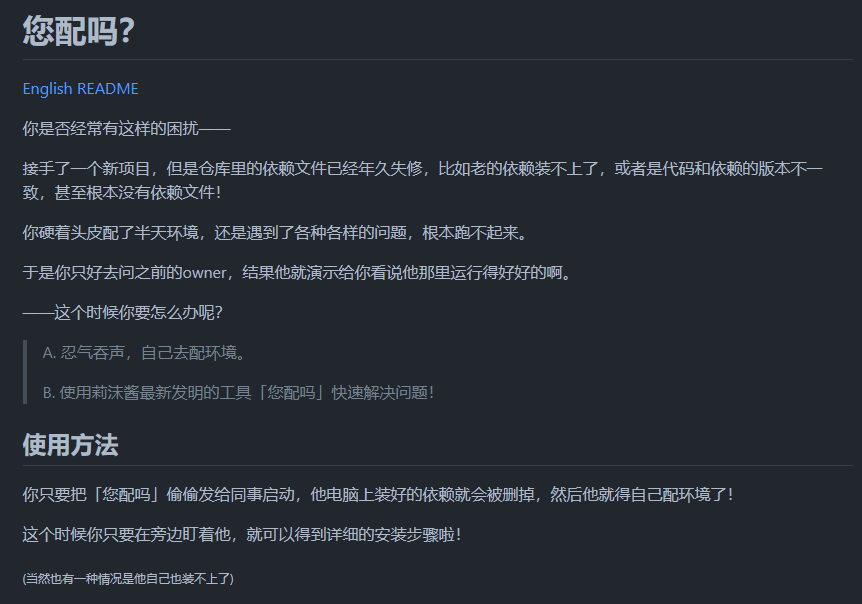
\includegraphics[width=0.90\linewidth]{pic/you-match.png}
\end{frame}

\begin{frame}{Docker 的作用}
    \begin{block}{Docker}
       Docker 将应用及其所需要的环境打包并交付给其他人使用, 使得应用能够在一致的环境下一键运行, 而不需要手动配置环境
    \end{block}
    \begin{block}{特点}
        \begin{itemize}
            \item 更高效的利用系统资源
            \item 更快速的启动时间
            \item 更方便持续交付和部署
        \end{itemize}
    \end{block}
\end{frame}


% 重要概念:镜像与容器
\begin{frame}{Docker 中的重要概念:镜像、容器与 Registry}
    \begin{block}{镜像(Image)}
        Docker 镜像是一个特殊的文件系统
        \begin{itemize}
            \item 提供容器运行时所需的程序、库、资源、配置等文件
            \item 包含一些为运行时准备的一些配置参数
            \item 不包含任何动态数据, 其内容在构建之后也不会被改变
        \end{itemize}
    \end{block}
\end{frame}

\begin{frame}{Docker 中的重要概念:镜像、容器与 Registry}
    \begin{block}{镜像(Image)}
        Docker 镜像的构建:Dockerfile 示例
        \begin{figure}
            \centering
            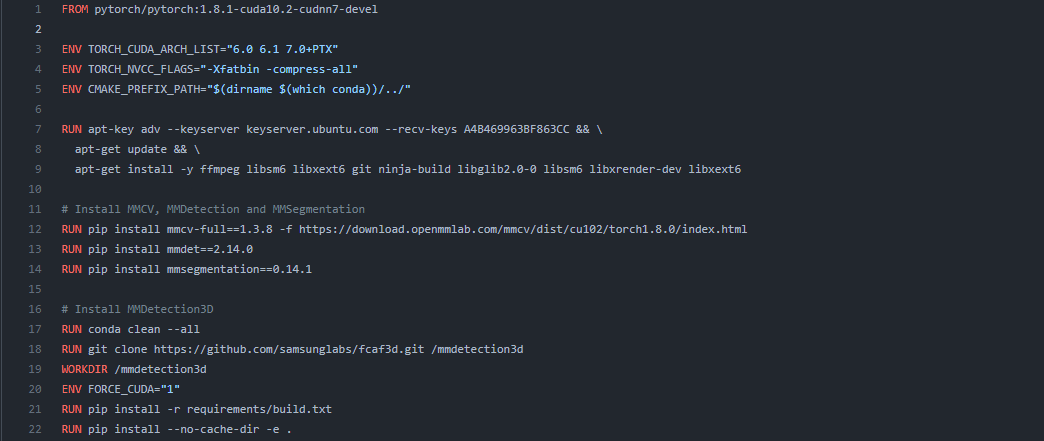
\includegraphics[width=0.80\textwidth]{pic/dockerfile-example.png}
            \label{fig:my_label}
        \end{figure}
        \begin{itemize}
            \item 语法规范详见:\url{https://yeasy.gitbook.io/docker_practice/image/dockerfile}
            \item 之后使用 docker build 命令构建镜像
        \end{itemize}
    \end{block}
\end{frame}


\begin{frame}{Docker 中的重要概念:镜像、容器与 Registry}
    \begin{block}{容器(Container)}
        \begin{itemize}
            \item 镜像的\textbf{实例}:镜像是静态的定义, 容器是镜像运行时的实体
            \item 具有\textbf{易失性}:任何保存于容器存储层的信息都会随容器删除而丢失(大作业需要将用户数据保存在持久化存储中)
        \end{itemize}
        容器的启动:
        \begin{itemize}
            \item (本地)docker run -itd -p 10001:8000 --name <Container Name> <Image>
            \item (其他部署工具)查阅对应文档...
        \end{itemize}
    \end{block}
\end{frame}


\begin{frame}{Docker 中的重要概念:镜像、容器与 Registry}
    \begin{block}{Registry}
        概念辨析:仓库(Repository)、注册服务器(Registry)
        \begin{itemize}
            \item 镜像构建完成后, 可以很容易的在当前宿主机上运行, 但是, 如果需要在其它服务器上使用这个镜像, 我们就需要一个集中的存储、分发镜像的服务, Docker Registry 就是这样的服务. 
            \item 一个 Docker Registry 中可以包含多个仓库(Repository);每个仓库可以包含多个标签(Tag);每个标签对应一个镜像. 
        \end{itemize}
    \end{block}
\end{frame}


\begin{frame}{Docker 中的重要概念:镜像、容器与 Registry}
    \begin{block}{Registry}
        \begin{figure}
            \centering
            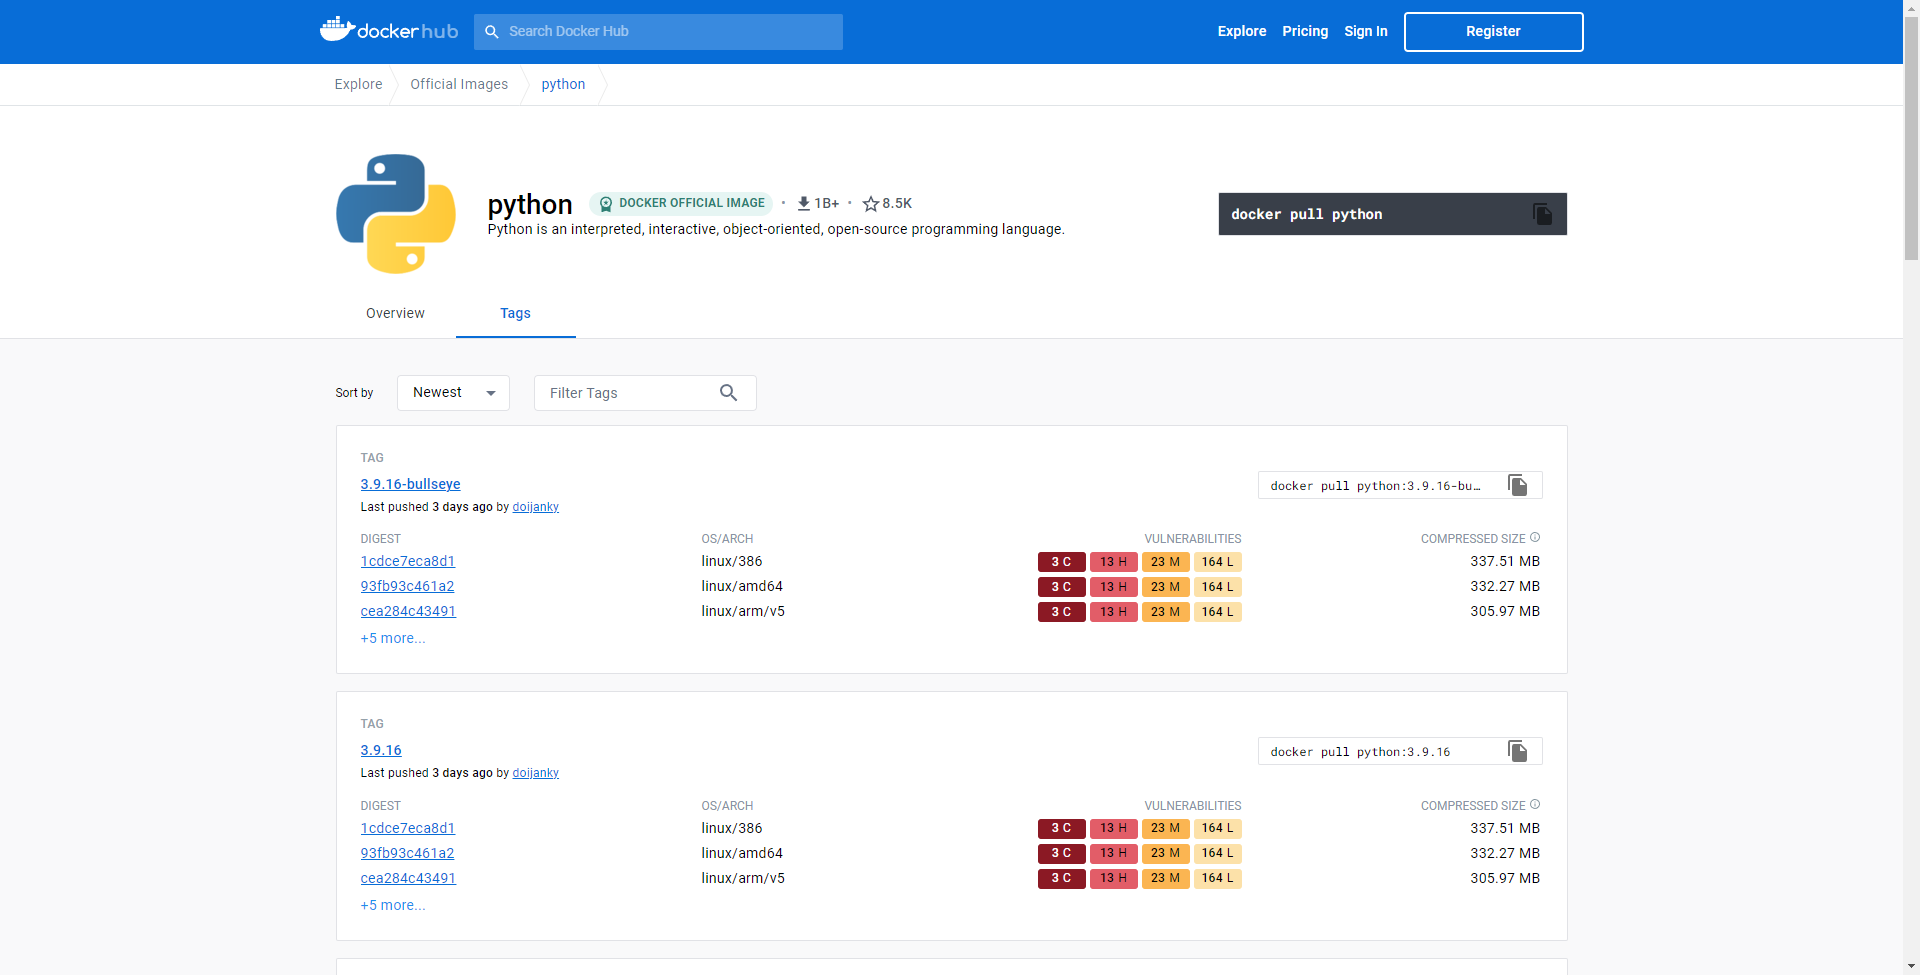
\includegraphics[width=1.00\textwidth]{pic/dockerhub.png}
            \caption{概念辨析:Docker Hub; 图中的 python;  python:3.9.16}
            \label{fig:my_label}
        \end{figure}

    \end{block}
\end{frame}

\begin{frame}{Dockerfile 编写入门}
参考 \href{https://thuse-course.github.io/course-index/deploy/docker/}{\textcolor{blue}{课程文档 Docker 部分}} 与 \href{https://summer23.net9.org/sast2023-docker/}{\textcolor{blue}{2023 酒井科协暑培 Docker 课程}}
\end{frame}

\section{持续集成与持续部署简介}

\begin{frame}{持续集成与持续部署}
    \begin{block}{持续集成 (Continuous Integration/CI)}
        \begin{itemize}
            \item 在代码构建过程中持续地进行代码的集成、构建、以及自动化测试等
            \item 可以在代码提交的过程中通过单元测试等尽早地发现引入的错误
        \end{itemize}
    \end{block}
    
    \begin{block}{持续部署 (Continuous Deployment/CD)}
        \begin{itemize}
            \item 在代码构建完毕后迅速将新版本部署上线
            \item 有利于快速迭代并交付产品
        \end{itemize}
    \end{block}
\end{frame}

\begin{frame}{持续集成与持续部署}
    \begin{block}{为什么需要 CI/CD}
        \begin{itemize}
            \item 自动化:不用手动执行测试、部署等
            \item 标准化:定义一套固定的流程, 避免人为部署带来的错误
            \item 尽早发现错误:避免长时间后难以定位问题根源
        \end{itemize}
    \end{block}
\end{frame}

\begin{frame}{GitLab CI/CD}
    \begin{block}{GitLab CI/CD}
        \begin{itemize}
            \item 一套基于 GitLab 的 CI/CD 系统
            \item 可以让开发人员通过 .gitlab-ci.yml 在项目中配置 CI/CD 流程
            \item 在每次 push 到仓库后, 系统都可以自动(或手动)地执行 CI/CD 所定义的操作
        \end{itemize}
    \end{block}
\end{frame}

\begin{frame}{基本概念}
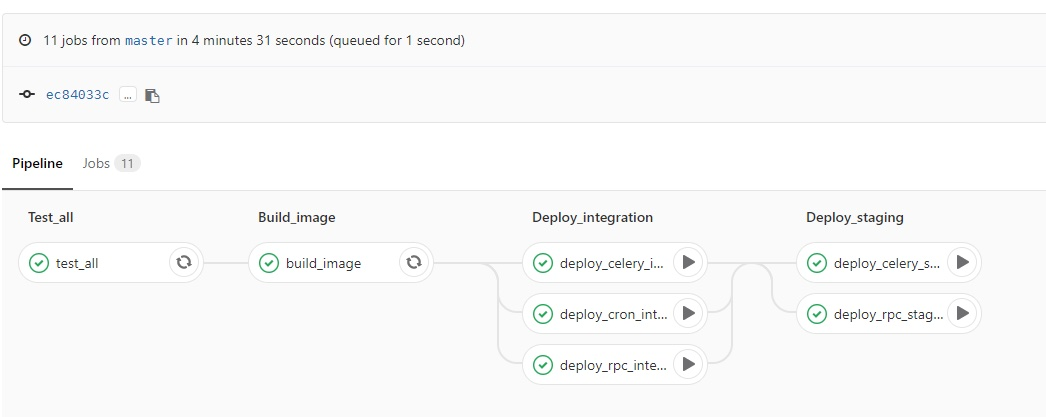
\includegraphics[width=0.90\linewidth]{pic/pipeline.jpg}
\end{frame}

\begin{frame}{基本概念}
    \begin{block}{作业 (Job)}
        \begin{itemize}
            \item  CI/CD 流程的最小执行单元
            \item 包含了一系列需要执行的命令
            \item 需要指定一个 Docker 镜像, 在执行 CI/CD 时将会基于此镜像运行一个容器, 在其中执行命令
            \item 成功状态将取决于其最后一条命令的返回值
        \end{itemize}
    \end{block}
\end{frame}

\begin{frame}{基本概念}
    \begin{block}{阶段 (Stage)}
        \begin{itemize}
            \item CI/CD 流程划分为多个阶段分别进行, 每个阶段可以包含一个或多个作业
            \item 同一个阶段的多个作业可以并行执行
            \item 一个阶段的所有作业均成功执行后, 才会执行下一个阶段的作业 时将会基于此镜像运行一个容器, 在其中执行命令
        \end{itemize}
    \end{block}
\end{frame}

\begin{frame}{基本概念}
    \begin{block}{流水线 (Pipeline)}
        \begin{itemize}
            \item 多个阶段顺序连接组成一个流水线
            \item 将代码推送到远程仓库或是发起合并请求时, GitLab 会基于该版本的代码执行流水线
        \end{itemize}
    \end{block}
\end{frame}

\begin{frame}{.gitlab-ci.yml}
    \begin{block}{镜像指定}
        \begin{lstlisting}
        a
        
            image: python:3.9
        \end{lstlisting}
    \end{block}
    \begin{block}{阶段定义}
        \begin{lstlisting}
        b
        
            stages:
            
            \ \ - build
            
            \ \ - test
            
            \ \ - deploy
        \end{lstlisting}
    \end{block}
\end{frame}

\begin{frame}{.gitlab-ci.yml}
    \begin{block}{作业定义}
        \begin{lstlisting}
        c
        
            style-test:
            
            \ \ stage: test
            
            \ 
            
            \ \ before\_script:
            
            \ \ \ \ - pip install pylint
            
            \ \ script:
            
            \ \ \ \ - pylint **/*.py
        \end{lstlisting}
    \end{block}
\end{frame}

\section{SECoder 平台简介}

\begin{frame}{SECoder}
    \centering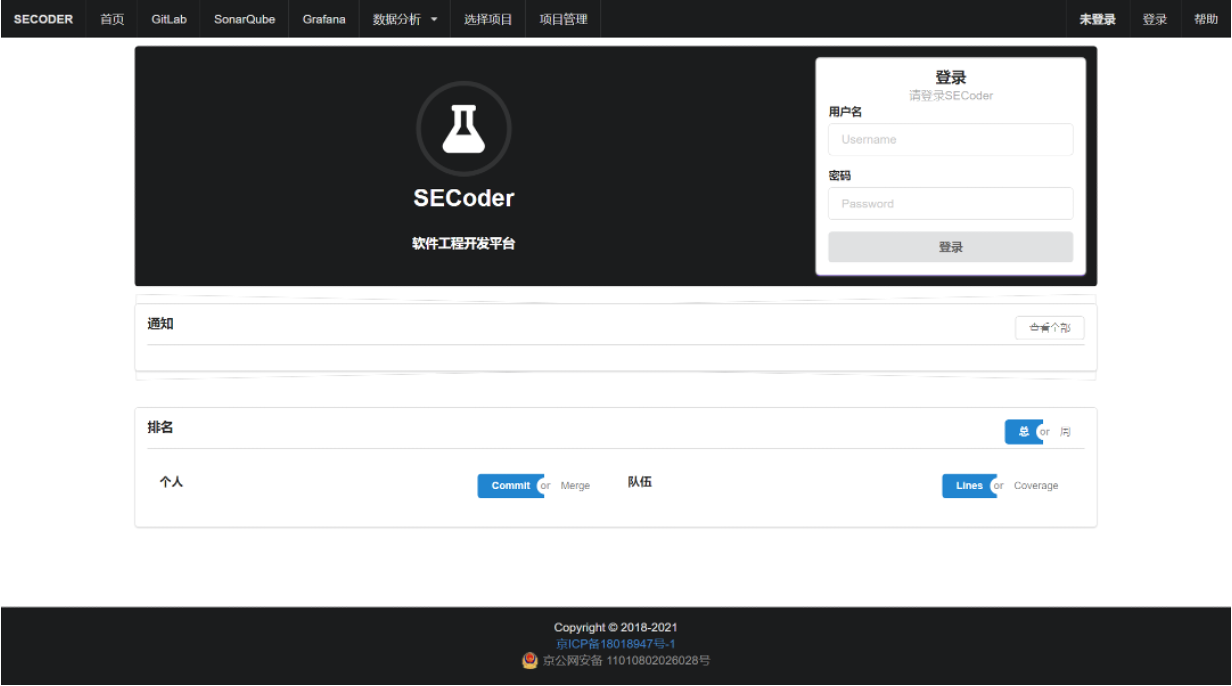
\includegraphics[width=0.75\linewidth]{pic/secoder.png}
    \begin{block}{软件工程开发平台 (SECoder)}
        \begin{itemize}
            \item 帮助同学们顺利完成软件工程课程大作业的在线网站, 提供了 GitLab、SonarQube 等用于更好管理开发流程的工具
            \item \url{https://sep.secoder.net}
        \end{itemize}
    \end{block}
\end{frame}

\begin{frame}{SECoder}
    \begin{minipage}{0.35\linewidth}
        \begin{block}{项目管理}
            \begin{itemize}
                \item 提交数量和质量
                \item 任务数量
                \item 各仓库代码行数
                \item 注释比例
                \item 构建成功率
                \item 测试覆盖率
            \end{itemize}
        \end{block}
    \end{minipage}
    \begin{minipage}{0.6\linewidth}
        \centering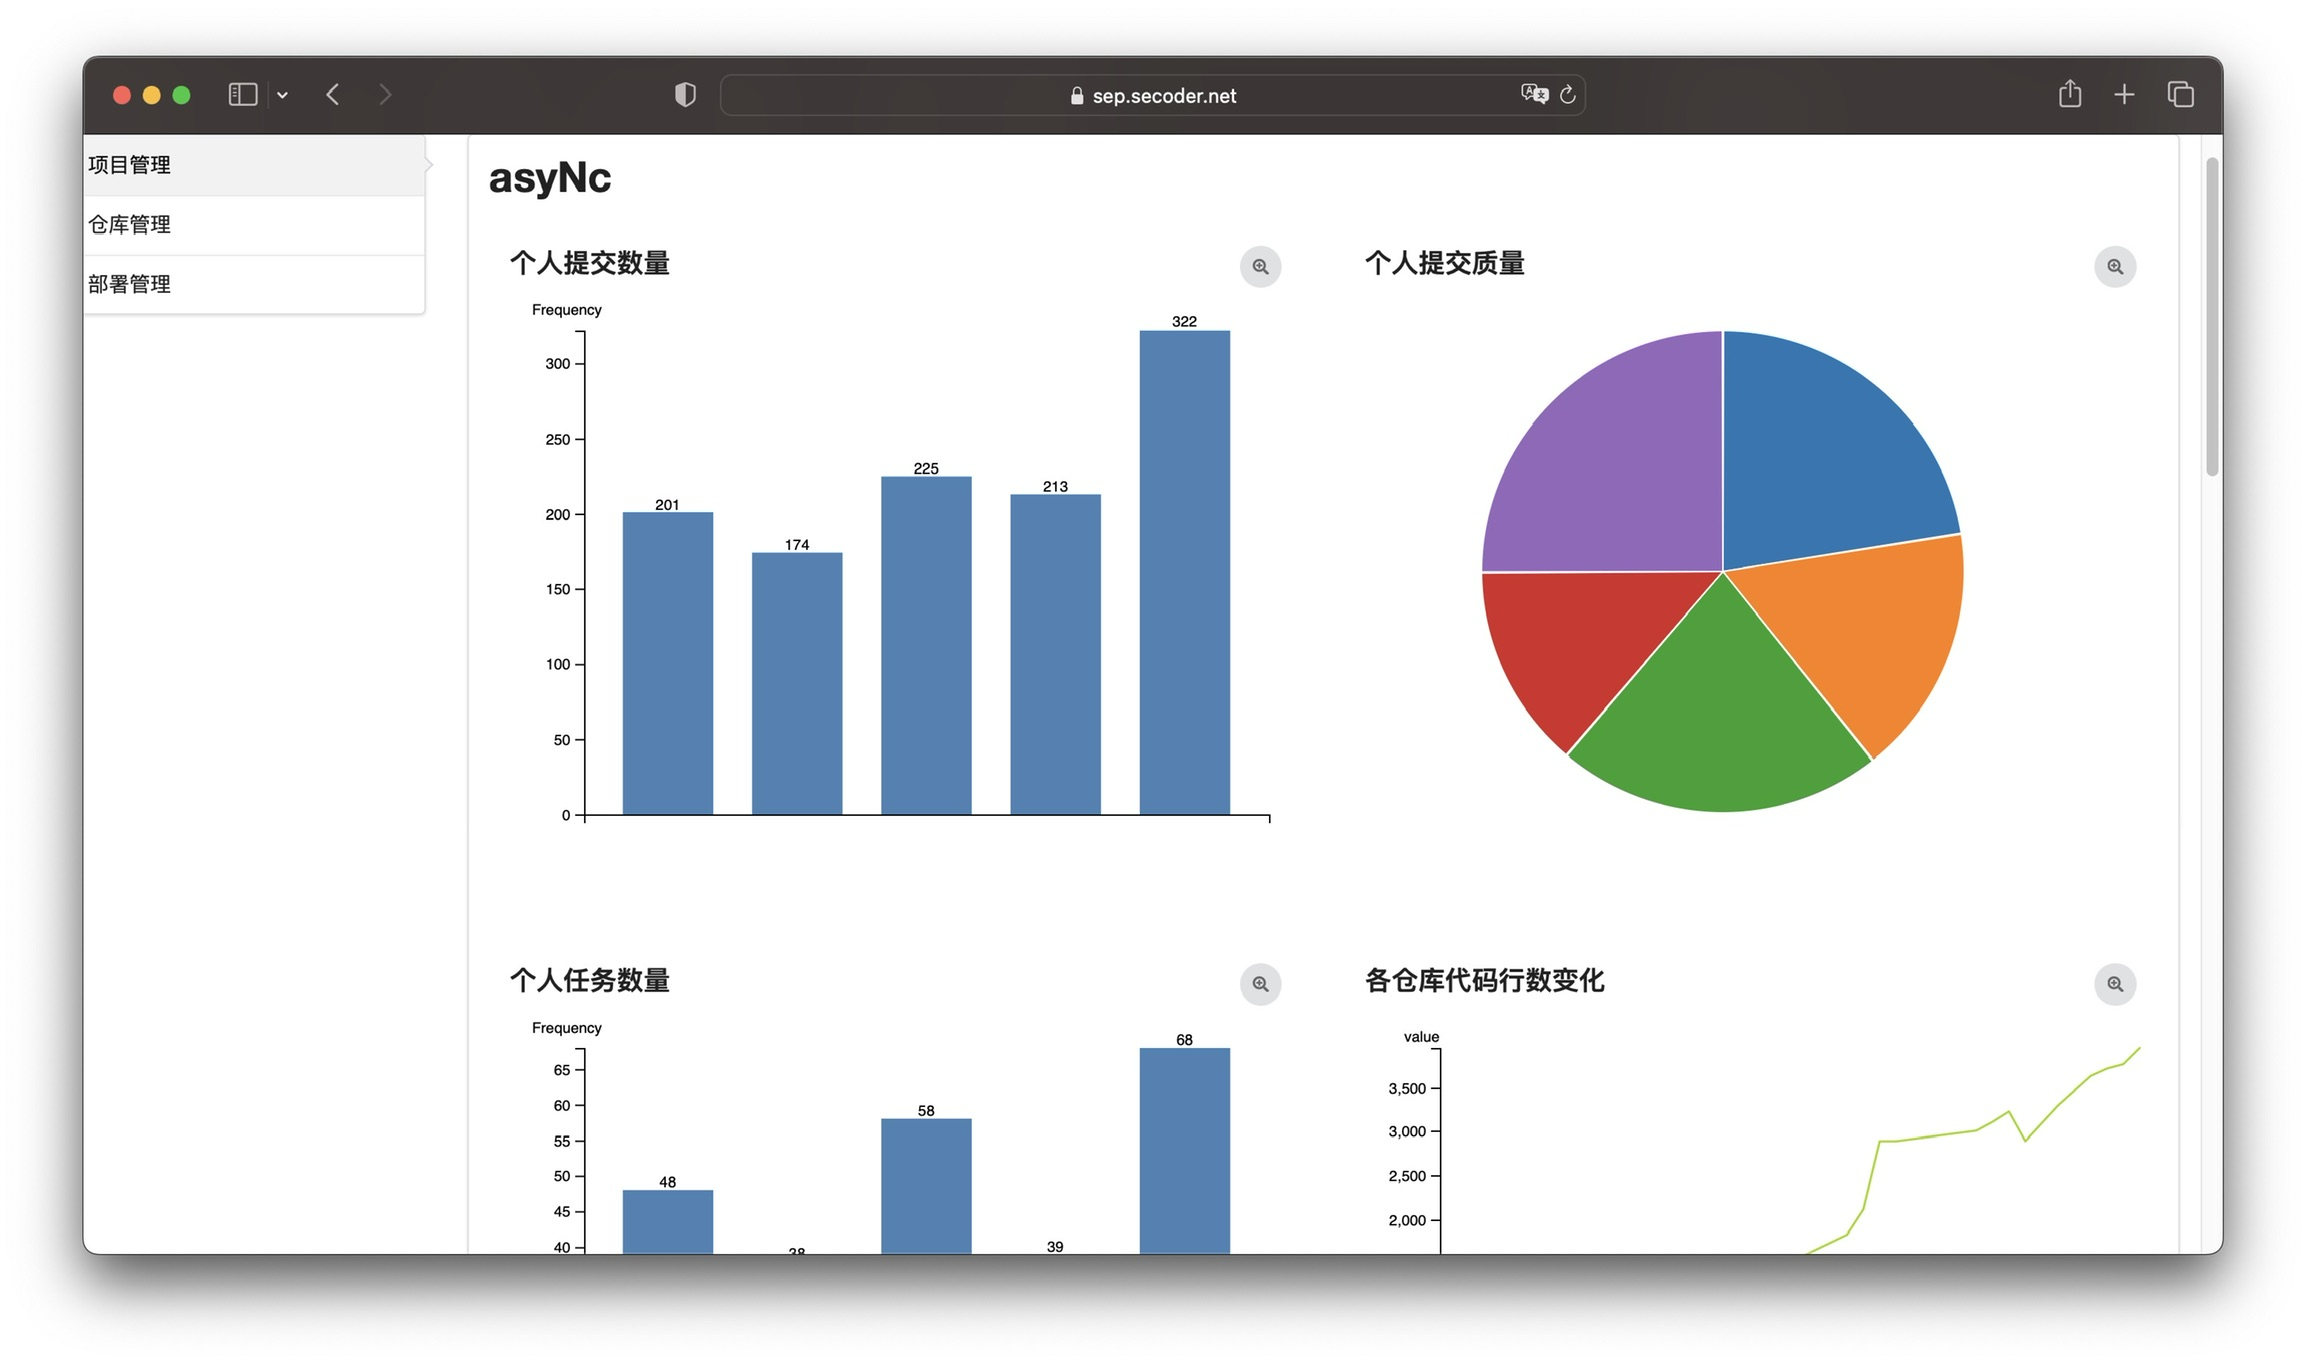
\includegraphics[width=1.0\linewidth]{pic/cake.jpg}
    \end{minipage}
\end{frame}

\begin{frame}{SECoder}
    \centering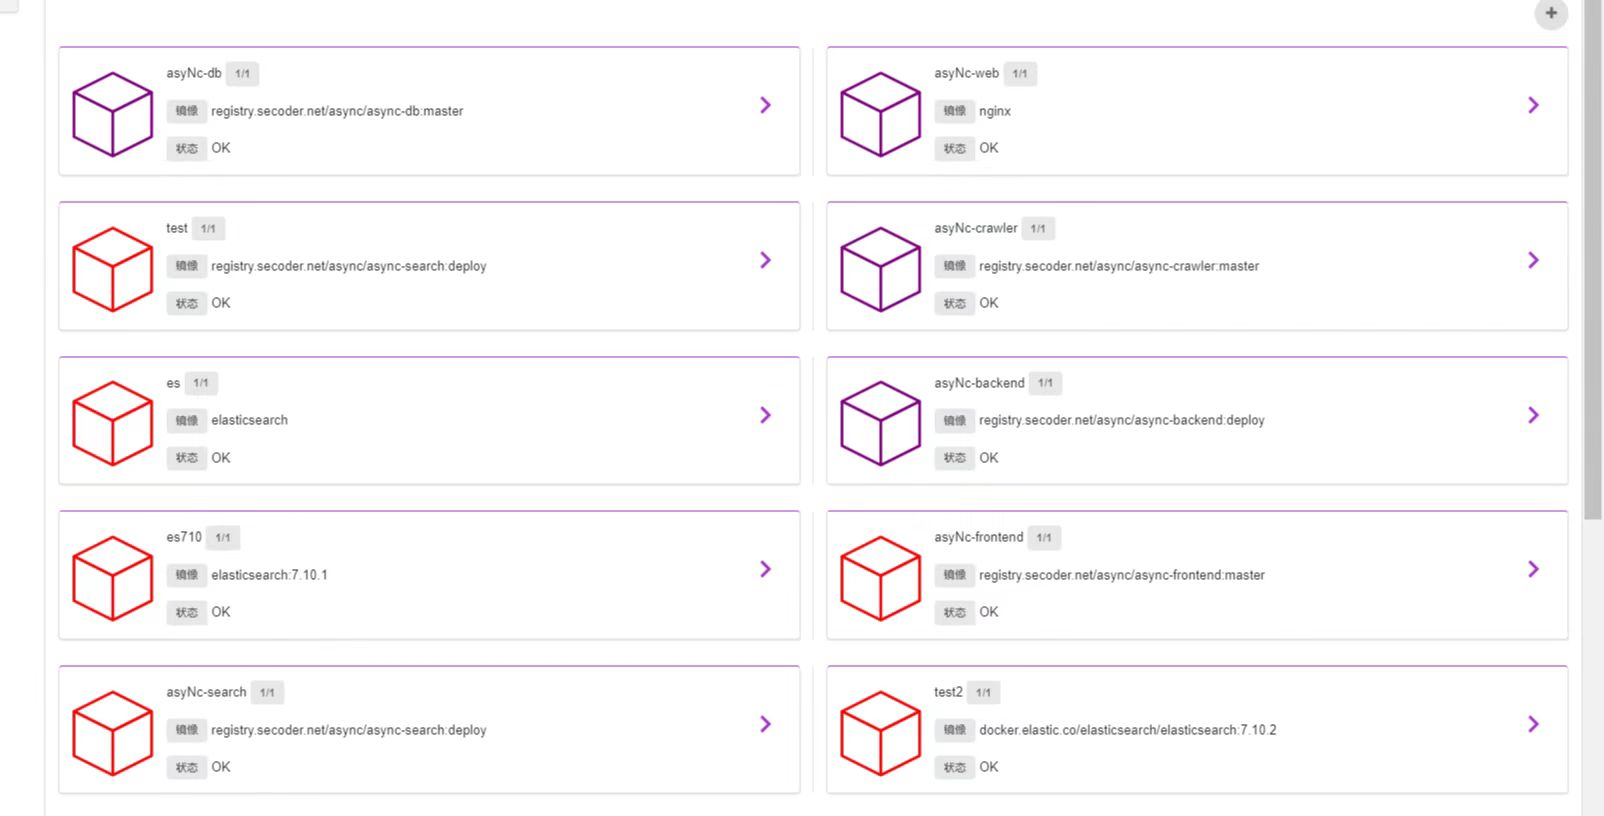
\includegraphics[width=0.7\linewidth]{pic/dynos.jpg}
    \begin{block}{部署管理}
        \begin{itemize}
        \item 对团队的容器进行各种管理操作
        \item 建立仓库时选择「启用部署」即可创建一个关联的容器
        \end{itemize}
    \end{block}
\end{frame}

\begin{frame}{SECoder}
    \begin{block}{配置项}
        \begin{itemize}
            \item 在开发时和正式部署时使用不同的配置是一种常见做法
            \item 然而, 由于容器的易失性, 一个容器在删除后其中所做的修改都将丢失
            \begin{itemize}\item 这意味着每次都手动修改配置会很麻烦
            \end{itemize}
            \item 可以通过配置项来简化这个流程
            \begin{itemize}\item 配置项是只读的挂载项, 可以用于存放各种配置文件
            \item 配置项可以作为一个目录被挂载到容器中
            \item 这样, 在部署时将会自动使用挂载的配置
            \end{itemize}
            \item 可参考文档中的 \href{https://thuse-course.github.io/course-index/deploy/secoder/\#\_12}{\underline{配置挂载演示}}
        \end{itemize}
    \end{block}
\end{frame}

\begin{frame}{SECoder}
    \begin{block}{持久存储}
        \begin{itemize}
            \item 数据库容器等需要在容器内保存数据
            \item 但同样由于容器的易失性, 在容器重启时其中的数据将会丢失, 因此我们需要一种能够持久保存数据的方法
            \item 持久存储与配置项类似, 都可以挂载到容器的某一目录
            \begin{itemize}\item 不同点在于持久存储是可写的, 并且你不需要为其提供初始内容
            \item 在不同的容器实例间保持数据
            \end{itemize}
            \item 操作步骤与配置项类似
            \item 可参考 SECoder 帮助文档中的  \href{https://docs.secoder.net/service/deployer/tutorial-database/}{\underline{数据库教程}}
        \end{itemize}
    \end{block}
\end{frame}

\begin{frame}
    \begin{center}
        {\Huge\calligra Thanks!} ~\\ ~\\ ~\\
        ~\\
        ~\\
        Questions?
    \end{center}
\end{frame}

\end{document}